\documentclass[12pt,a4paper]{article}

\usepackage[utf8]{inputenc}
\usepackage{graphicx}
\usepackage[spanish]{babel}
\usepackage{float}				%Para poner las imagenes exactamente donde se me cante las pelotas en caso de quererlo, poniendole [H]
\usepackage{amsmath}
\usepackage{epstopdf}
\usepackage{geometry}
\usepackage{hieroglf}
\usepackage{subcaption}
\usepackage[justification=centering]{caption}
\usepackage[colorlinks=true, allcolors=blue]{hyperref}
\geometry{
a4paper,
left=20mm,
right=20mm,
top=25mm,
bottom = 20mm
}
\usepackage{float}
\usepackage{units}
\marginparwidth=2cm
\usepackage[colorinlistoftodos]{todonotes}

% \usepackage{hyperref}   %Esto es para ir a los links

\title{\mathbf{Mecánica de Medios Continuos \\Práctica 5 \\ Ecuaciones de conservación-Balance}}

\author{Universidad de Cuenca}
\begin{document}
\maketitle
\begin{enumerate}
    \item Teorema de transporte de Reynolds.
    \begin{enumerate}
        \item \textbf{Lema de Reynolds.}  Demostrar el lema de Reynolds (Ecuación \ref{eq:LemaR}). Pista: $dV_t=\det{(\mathbf{F})}dV_0$ y  $\frac{d\det{(\mathbf{F})}}{dt}=\det{(\mathbf{F})}\nabla\cdot \mathbf{v}$
        \begin{equation}  \label{eq:LemaR}
            \frac{d}{dt}\int_{V_t=V}\rho\phi dV=\int_{V}\rho\frac{d\phi}{dt}dV
        \end{equation}
        
        \item \textbf{Derivada  material de una integral de volumen.} De manera similar al punto anterior, demostrar la siguiente igualdad:
        \begin{equation}
            \frac{d}{dt}\int_{V_t=V}\mu(\mathbf{x},t)dV=\frac{\partial}{\partial t}\int_{V}\mu dV + \int_{V}\nabla\cdot(\mu \mathbf{v})dV            
        \end{equation}
        \item Combinando los resultados de los items anteriores, demostrar el \textbf{Teorema de Transporte de Reynolds}
    \end{enumerate}
\item Considerar un chorro de líquido incompresible, irrotacional, y de sección uniforme $\beta$ que choca con una pared, como se muestra en la figura \ref{fig:chorro}. El chorro se divide en dos corrientes de secciones uniformes $\beta_1$ y $\beta_2$.
\begin{enumerate}
    \item Calcular estas secciones considerando que no actúan fuerzas externas.
    \item ¿Cuál es la fuerza ejercida por el chorro sobre la pared?
    \begin{figure}
        \centering  
        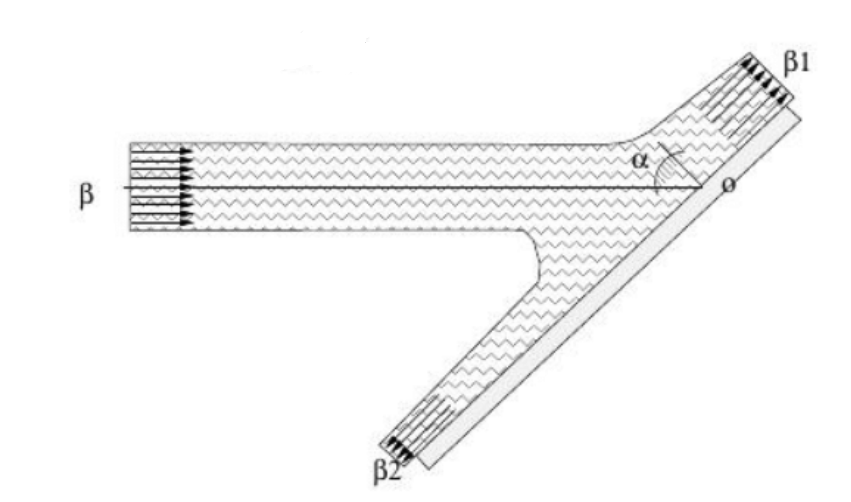
\includegraphics[width=0.5\textwidth]{tp5-1.png}    
        \caption{ }\label{fig:chorro}
    \end{figure}
    \end{enumerate}
\end{enumerate}
\end{document}